%%%%%%%%%%%%%%%%%%%%%%%%%%%%%%%%%%%%%%%%%%%%%%%%%%%%%%%%%%%%%%%%%%
%%%%%%%% ICML 2010 EXAMPLE LATEX SUBMISSION FILE %%%%%%%%%%%%%%%%%
%%%%%%%%%%%%%%%%%%%%%%%%%%%%%%%%%%%%%%%%%%%%%%%%%%%%%%%%%%%%%%%%%%

% Use the following line _only_ if you're still using LaTeX 2.09.
%\documentstyle[icml2010,epsf,natbib]{article}
% If you rely on Latex2e packages, like most moden people use this:
\documentclass{article}

% For figures
\usepackage{graphicx} % more modern
%\usepackage{epsfig} % less modern
\usepackage{subfigure} 

% For citations
\usepackage{natbib}

% For algorithms
\usepackage{algorithm}
\usepackage{algorithmic}

% As of 2010, we use the hyperref package to produce hyperlinks in the
% resulting PDF.  If this breaks your system, please commend out the
% following usepackage line and replace \usepackage{icml2010} with
% \usepackage[nohyperref]{icml2010} above.
\usepackage{hyperref}

% Packages hyperref and algorithmic misbehave sometimes.  We can fix
% this with the following command.
\newcommand{\theHalgorithm}{\arabic{algorithm}}

% Employ the following version of the ``usepackage'' statement for
% submitting the draft version of the paper for review.  This will set
% the note in the first column to ``Under review.  Do not distribute.''
\usepackage{icml2010} 
% Employ this version of the ``usepackage'' statement after the paper has
% been accepted, when creating the final version.  This will set the
% note in the first column to ``Appearing in''
% \usepackage[accepted]{icml2010}

%%%%%%% start commands
\newcommand{\mA}{\mathcal{A}}
\newcommand{\mB}{\mathcal{B}}
\newcommand{\mC}{\mathcal{C}}
\newcommand{\mD}{\mathcal{D}}
\newcommand{\mE}{\mathcal{E}}
\newcommand{\mF}{\mathcal{F}}
\newcommand{\mG}{\mathcal{G}}
\newcommand{\mH}{\mathcal{H}}
\newcommand{\mI}{\mathcal{I}}
\newcommand{\mJ}{\mathcal{J}}
\newcommand{\mK}{\mathcal{K}}
\newcommand{\mL}{\mathcal{L}}
\newcommand{\mM}{\mathcal{M}}
\newcommand{\mN}{\mathcal{N}}
\newcommand{\mO}{\mathcal{O}}
\newcommand{\mP}{\mathcal{P}}
\newcommand{\mQ}{\mathcal{Q}}
\newcommand{\mR}{\mathcal{R}}
\newcommand{\mS}{\mathcal{S}}
\newcommand{\mT}{\mathcal{T}}
\newcommand{\mU}{\mathcal{U}}
\newcommand{\mV}{\mathcal{V}}
\newcommand{\mW}{\mathcal{W}}
\newcommand{\mX}{\mathcal{X}}
\newcommand{\mY}{\mathcal{Y}}
\newcommand{\mZ}{\mathcal{Z}}

\newcommand{\hmA}{\widehat{\mathcal{A}}}
\newcommand{\hmB}{\widehat{\mathcal{B}}}
\newcommand{\hmC}{\widehat{\mathcal{C}}}
\newcommand{\hmD}{\widehat{\mathcal{D}}}
\newcommand{\hmE}{\widehat{\mathcal{E}}}
\newcommand{\hmF}{\widehat{\mathcal{F}}}
\newcommand{\hmG}{\widehat{\mathcal{G}}}
\newcommand{\hmH}{\widehat{\mathcal{H}}}
\newcommand{\hmI}{\widehat{\mathcal{I}}}
\newcommand{\hmJ}{\widehat{\mathcal{J}}}
\newcommand{\hmK}{\widehat{\mathcal{K}}}
\newcommand{\hmL}{\widehat{\mathcal{L}}}
\newcommand{\hmM}{\widehat{\mathcal{M}}}
\newcommand{\hmN}{\widehat{\mathcal{N}}}
\newcommand{\hmO}{\widehat{\mathcal{O}}}
\newcommand{\hmP}{\widehat{\mathcal{P}}}
\newcommand{\hmQ}{\widehat{\mathcal{Q}}}
\newcommand{\hmR}{\widehat{\mathcal{R}}}
\newcommand{\hmS}{\widehat{\mathcal{S}}}
\newcommand{\hmT}{\widehat{\mathcal{T}}}
\newcommand{\hmU}{\widehat{\mathcal{U}}}
\newcommand{\hmV}{\widehat{\mathcal{V}}}
\newcommand{\hmW}{\widehat{\mathcal{W}}}
\newcommand{\hmX}{\widehat{\mathcal{X}}}
\newcommand{\hmY}{\widehat{\mathcal{Y}}}
\newcommand{\hmZ}{\widehat{\mathcal{Z}}}

\newcommand{\ha}{\widehat{a}}
\newcommand{\hb}{\widehat{b}}
\newcommand{\hc}{\widehat{c}}
\newcommand{\hd}{\widehat{d}}
\newcommand{\he}{\widehat{e}}
\newcommand{\hf}{\widehat{f}}
\newcommand{\hg}{\widehat{g}}
\newcommand{\hh}{\widehat{h}}
\newcommand{\hi}{\widehat{i}}
\newcommand{\hj}{\widehat{j}}
\newcommand{\hk}{\widehat{k}}
\newcommand{\hl}{\widehat{l}}
\newcommand{\hm}{\widehat{m}}
\newcommand{\hn}{\widehat{n}}
\newcommand{\ho}{\widehat{o}}
\newcommand{\hp}{\widehat{p}}
\newcommand{\hq}{\widehat{q}}
\newcommand{\hr}{\widehat{r}}
\newcommand{\hs}{\widehat{s}}
%\newcommand{\ht}{\widehat{t}}
\newcommand{\hu}{\widehat{u}}
\newcommand{\hv}{\widehat{v}}
\newcommand{\hw}{\widehat{w}}
\newcommand{\hx}{\widehat{x}}
\newcommand{\hy}{\widehat{y}}
\newcommand{\hz}{\widehat{z}}

\newcommand{\hA}{\widehat{A}}
\newcommand{\hB}{\widehat{B}}
\newcommand{\hC}{\widehat{C}}
\newcommand{\hD}{\widehat{D}}
\newcommand{\hE}{\widehat{E}}
\newcommand{\hF}{\widehat{F}}
\newcommand{\hG}{\widehat{G}}
\newcommand{\hH}{\widehat{H}}
\newcommand{\hI}{\widehat{I}}
\newcommand{\hJ}{\widehat{J}}
\newcommand{\hK}{\widehat{K}}
\newcommand{\hL}{\widehat{L}}
\newcommand{\hM}{\widehat{M}}
\newcommand{\hN}{\widehat{N}}
\newcommand{\hO}{\widehat{O}}
\newcommand{\hP}{\widehat{P}}
\newcommand{\hQ}{\widehat{Q}}
\newcommand{\hR}{\widehat{R}}
\newcommand{\hS}{\widehat{S}}
\newcommand{\hT}{\widehat{T}}
\newcommand{\hU}{\widehat{U}}
\newcommand{\hV}{\widehat{V}}
\newcommand{\hW}{\widehat{W}}
\newcommand{\hX}{\widehat{X}}
\newcommand{\hY}{\widehat{Y}}
\newcommand{\hZ}{\widehat{Z}}

\newcommand{\bA}{\mathbf{A}}
\newcommand{\bB}{\mathbf{B}}
\newcommand{\bC}{\mathbf{C}}
\newcommand{\bD}{\mathbf{D}}
\newcommand{\bE}{\mathbf{E}}
\newcommand{\bF}{\mathbf{F}}
\newcommand{\bG}{\mathbf{G}}
\newcommand{\bH}{\mathbf{H}}
\newcommand{\bI}{\mathbf{I}}
\newcommand{\bJ}{\mathbf{J}}
\newcommand{\bK}{\mathbf{K}}
\newcommand{\bL}{\mathbf{L}}
\newcommand{\bM}{\mathbf{M}}
\newcommand{\bN}{\mathbf{N}}
\newcommand{\bO}{\mathbf{O}}
\newcommand{\bP}{\mathbf{P}}
\newcommand{\bQ}{\mathbf{Q}}
\newcommand{\bR}{\mathbf{R}}
\newcommand{\bS}{\mathbf{S}}
\newcommand{\bT}{\mathbf{T}}
\newcommand{\bU}{\mathbf{U}}
\newcommand{\bV}{\mathbf{V}}
\newcommand{\bW}{\mathbf{W}}
\newcommand{\bX}{\mathbf{X}}
\newcommand{\bY}{\mathbf{Y}}
\newcommand{\bZ}{\mathbf{Z}}

\newcommand{\del}{\delta}
\newcommand{\sig}{\sigma}
\newcommand{\lam}{\lambda}
\newcommand{\gam}{\gamma}
\newcommand{\eps}{\varepsilon}

\newcommand{\Del}{\Delta}
\newcommand{\Sig}{\Sigma}
\newcommand{\Lam}{\Lambda}
\newcommand{\Gam}{\Gamma}

\newcommand{\halpha}{\widehat{\alpha}}
\newcommand{\hbeta}{\widehat{\beta}}
\newcommand{\hdel}{\widehat{\delta}}
\newcommand{\hsig}{\widehat{\sigma}}
\newcommand{\hlam}{\widehat{\lambda}}
\newcommand{\hgam}{\widehat{\gamma}}
\newcommand{\heeta}{\widehat{\eta}}
\newcommand{\homega}{\widehat{\omega}}
\newcommand{\hpi}{\widehat{\pi}}
\newcommand{\hmu}{\widehat{\mu}}
\newcommand{\hpsi}{\widehat{\psi}}
\newcommand{\heps}{\widehat{\eps}}
\newcommand{\hth}{\widehat{\theta}}

\newcommand{\hDel}{\widehat{\Delta}}
\newcommand{\hSig}{\widehat{\Sigma}}
\newcommand{\hLam}{\widehat{\Lambda}}
\newcommand{\hGam}{\widehat{\Gamma}}
\newcommand{\hPi}{\widehat{\Pi}}

\newcommand{\MeB}{\mM \overset{\varepsilon}{{\sim}}_F \mB}
\newcommand{\Real}{\mathbb{R}}
\newcommand{\conv}{\rightarrow}
\providecommand{\norm}[1]{\left \lVert#1 \right  \rVert}
\newcommand{\mED}{\mE_{\Delta}}
\newcommand{\hLD}{$\hLam_{\Delta}$}
\newcommand{\hbD}{\widehat{\mathbf{D}}}


%%%%%%% end commands


%%%%%% start packages
\usepackage{amsfonts}
\usepackage{amsmath}


%%%%%% end packages


% The \icmltitle you define below is probably too long as a header.
% Therefore, a short form for the running title is supplied here:
\icmltitlerunning{Submission and Formatting Instructions for ICML 2010}

\begin{document} 

\twocolumn[
\icmltitle{On utilizing structure to classify brain-graphs according to mental properties}

% It is OKAY to include author information, even for blind
% submissions: the style file will automatically remove it for you
% unless you've provided the [accepted] option to the icml2010
% package.
\icmlauthor{Your Name}{email@yourdomain.edu}
\icmladdress{Your Fantastic Institute,
            314159 Pi St., Palo Alto, CA 94306 USA}
\icmlauthor{Your CoAuthor's Name}{email@coauthordomain.edu}
\icmladdress{Their Fantastic Institute,
            27182 Exp St., Toronto, ON M6H 2T1 CANADA}

% You may provide any keywords that you 
% find helpful for describing your paper; these are used to populate 
% the "keywords" metadata in the PDF but will not be shown in the document
\icmlkeywords{boring formatting information, machine learning, ICML}

\vskip 0.3in
]

\begin{abstract} 
abstract
\end{abstract} 

\section{Introduction} % (fold)
\label{sec:introduction}


\paragraph{motivation}

The statistical analysis of populations of data that are well represented by networks is a rapidly developing field \cite{??}.  In particular, many aspects of the world, including economics, telecommunications, social websites, and transportation grids, to name a few, are well characterized by networks, or \emph{graphs}. While much work has been devoted to studying the statistics of individual graphs, less attention has been given to the analysis of populations of graphs.  Our interest here is to develop a number of classifiers that operate directly on graphs.  In our motivating example, the graphs correspond to brains of individuals, and mental properties of those individuals are the desired classifier output.  Because the aspects of these brain-graphs relevant for the classification task at hand is often unknown, a priori, we build a number of different classifiers, each designed to be optimal under certain model assumptions.  We show that classification performance increases as the number of training exemplars increases, and each algorithm outperforms the others when the data that is classified is generated from the assumed model.  This suggests that these tools provide not only a novel mechanism for classifying graphs, but also a guide for understanding the mechanism underlying the different classes.  


% \paragraph{graph theory background}
% 
% erdos-renyi, p1, ERGM, stochastic blockmodels, latent feature models, graph classifiers
% 
% \paragraph{brains as graphs background}
% 
% old skool: cajal, neural networks, PDP, 
% new skool: sporns and refs
% 
% \paragraph{outline}


The rest of the manuscript is organized as follows....  %Section \ref{sec:def} rigorously defines the mathematical objects under investigating.  Section \ref{sec:alg} develops a number of algorithms which are proven to be asymptotically optimal under various model assumptions.  The performance of these algorithms under various simulated modeling assumptions is demonstrated in Section \ref{sec:results}.  Finally, Section \ref{sec:discussion} discusses some potential ramifications of these results, and possible directions for future work.

% section introduction (end)

\section{Definitions} % (fold)
\label{sec:def}

Our intention is to build classifiers the operate on graphs.  To proceed, we rigorous define the mathematical objects under investigation.

\subsection{Mental Properties} % (fold)
\label{sub:mental_properties}

By ``mental property'', we mean one of many possible mental properties, including intelligence level, knowledge of a certain fact or set of facts, skill level, etc.  We will investigate the relationship between brains and a \emph{single} mental property here, and leave multiple categorical classifications to future work.  Let $\mM$ be the space of all mental properties under investigation, so that $m \in \mM$.  We restrict our work here to two-way classifications, so $\mM=\{0,1\}$, corresponding to having/not having some property, or having an ability over some threshold, etc.  

% section mental_properties (end)

\subsection{Brain-graphs} % (fold)
\label{sub:brain_graphs}


With this in mind, we propose the notion of a \emph{brain-graph}. Specifically, we say that the brain may be well characterized as a labeled, attributed multigraph (which is a generalized notion of a or network). Formally, we define a brain-graph, $b\in \mB$ as a triple, $\mB=(\mV,\mA,\mX)$, defined by the following:
\begin{itemize}
	\item The set of vertices (nodes), $V=\{V_i\}_{i\in[N]} \in \mV \subseteq \mathbb{Z}$, where $V_i \in \{0,1\}$ for $i \in [N]=\{1,2,\ldots,N\}$, and  $\mathbb{Z}$ is the set of integers, $\{0,1,2,\ldots\}$.  
	\item The set of arcs (edges), $A=\{A_{ij}\}_{i,j \in [N]} \in \mE \subseteq \mathbb{Z}^{N^2}$. Implicitly, the above definition allows for multiedges, i.e.,  $A_{ij}: \Omega \mapsto \mathbb{Z}\, \forall \, i,j$.  For clarity, we restict this notion of multiedges to integer \emph{edge weights}, not categorically different edges.  Thus, the phrase  ``number of edges'' will always refer to elements of the matrix $A$, and not number of edges between a particular pair of vertices.  
	\item The set of vertex features, $X=\{X_i\}_{i\in[N]} \in \mX \subseteq \Real^{d \times N}$, and $d$ is the countable dimensionality of the feature vectors. These vertex features may or may not be observed.
\end{itemize}

Throughout, we assume $n$ is known a priori, and the vertices are \emph{labeled}.  Further, we assume that both edges and features are random variables, but only edges are observed.  Thus, we denote a random brain-graph $b=(a,x)$, where $a=\{a_{ij}\}_{i,j \in [N]}$, and $x=\{x_i^k\}_{i\in[N], k \in [d]}$.  The class-conditional probability distributions are therefore be defined by $F_{B|M}=P[B | M]=P[A,X|M]$.  


% section brain_graphs (end)
% section definitions (end)

\section{Simulation} % (fold)
\label{sec:simulation}

To generate data to assess our brain-graph classifiers, we consider a species whose nervous system consists of the same (small) number of labeled neurons for each organism. {\it Caenorhabditis elegans} is believed to be such a species \cite{Durbin87}. The hermaphroditic C.~elegans' somatic nervous system consists of 279 interconnected neurons. While the graph with these neurons as vertices and edges defined by chemical synapses between neurons is not identical across individuals, it is reasonably consistent \cite{Durbin87}. Furthermore, these animals exhibit a rich behavioral repertoire that depends on circuit properties \cite{deBonoMaricq05}. Thus, one may design an experiment by describing the joint distribution $F_{BM}$ via class-conditional distributions $F_{B|M=m_j}$ for the C.~elegans brain-graph for two mental properties of interest, $m_0$ and $m_1$, along with the prior probability of class membership $P[M=m_1]$. Here the mental property corresponds to the C.~elegans exhibiting or not exhibiting a particular behavior (e.g., response to an odor).

%Simulations suggest that one may build a classifier, practically and with a manageable training sample size $n$, that demonstrates $\varepsilon$-supervenience with reasonable choices for $\varepsilon$ and $\alpha$ and a plausible joint distribution $F_{BM}$ (Figure \ref{fig1}). 
To generate the data, we let the class-conditional random variable $A_{ij} | M=m_0$ be distributed Poisson$(E_{ij}+\eta)$, where $E_{ij}$ is the number of chemical synapses between neuron $i$ and neuron $j$ according to \cite{VarshneyChklovskii09}, with noise parameter $0<\eta \ll 1$. The class-conditional random variable $A_{ij} | M=m_1$ is distributed Poisson$(E_{ij}+ \varepsilon_{ij})$ for neurons $i,j \in \mED$, where $\mED$ is the set of edges deemed responsible for odor-evoked behavior according to \cite{ChalasaniBargmann07}, with signal parameter $\varepsilon_{ij}$ uniformly sampled from $[-5,5]$. %We consider $k_n$-nearest neighbor classification of labeled multigraphs (directed, with loops) on 279 vertices, under Frobenius norm. The $k_n$-nearest neighbor classifier used here satisfies $k_n \rightarrow \infty$ as $n \rightarrow \infty$ and $k_n/n \rightarrow 0$ as $n \rightarrow \infty$, ensuring universal consistency. (Better classifiers can be constructed for the joint distribution $F_{BM}$ used here; however, we demand universal consistency.)

%Importantly, conducting this experiment {\it in actu} is not beyond current technological limitations. 3D superresolution imaging \cite{VaziriShank08} combined with neurite tracing algorithms \cite{HelmstaedterDenk08,Mishchenko09,LuLichtman09} allow the collection of a brain-graph within a day. Genetic manipulations, laser ablations, and training paradigms can each be used to obtain a non-wild type population for use as $M=m_1$ \cite{deBonoMaricq05}, and the class of each organism ($m_0$ vs.~$m_1$) can also be determined automatically \cite{BuckinghamSattelle08}.



% section simulation (end)


\section{Classifiers} % (fold)
\label{sec:classifiers}

If we knew $F_{B|0}$ and $F_{B|1}$, then classification would be trivial, let $\hm=\arg \max_{m} F_{B|m}$.   However, in practice these distributions are typically unknown. Therefore, we must estimate $g$ from a corpus data. Assume we have collected $N$ brain/mental pairs. Then, define the corpus of data as the collection of all such pairs: $\mD_{N}=\{(b_1,m_1), \ldots, (b_n,m_n)\}$. The estimated classifier, $\hg$, then takes a new brain and the old \emph{training data}, and makes predictions about the mental property $m$. Formally, $\hg: \mB \times (\mB, \mM)^n \mapsto \mM$, so $\hg(b; \mD_n)=\hm$.  The goal is to find the classifier, $\hg \in \mG$, that minimizes some loss function, $L$, given the data.  For two-way classification, a potentially reasonable loss function is $L_F(\hg)=\mathbb{E}[P_F(\hg(B;\mD_n) \neq M | \mD_n)]$.  

Below, we describe several different graph classification algorithms that we will apply to simulated data.  Each algorithm is built explicitly with some model assumptions in mind.  As the number of constraints increase, the bias of the classifier potentially increases.  However, the variance certainly decreases.  So, if we can find an algorithm that reduces the variance more than it increases the bias, then we win the bias-variance trade-off, and have obtained the best $\hg$ we can find.  Further, comparing the various algorithmic performances' on real data will inform us with regard to which model assumptions are best supported by the data, potentially leading to greater insight and understanding of the underlying neurobiology.  


\section{$k_n$ nearest neighbor (kNN)} % (fold)
\label{sub:_k_n_nearest_neighbor_knn_}

The $k_n$ nearest neighbor (kNN) algorithm was proven to be universally consistent when the data are vectors in $\Real^d$ \cite{Stone77}.  More recently, Vogelstein et al. (2009) extended this proof to the space of attributed multigraphs \cite{VVP09}.  Universality implies that no matter what $F_{B|M}$ looks like, the kNN algorithm will asymptotically converge to the Bayes optimal estimator, that is, as $N\conv\infty$, $\hg \conv g_{\ast}$, where $g_{\ast}= \arg \max_{g\in\mG} L_F(g)$.  

The kNN algorithm on graphs operates as follows.  Let $d(b_i,b_j)=\norm{a_i,a_j}_F^2$, where $a_i$ is the adjacency matrix for brain $i$.  Given a new brain, $b$, compute $d(b,b_i)\, \forall i \in [n]$.  Then, sort the brains and their corresponding mental properties according to their distances from $b$: $b_{(1)}, b_{(2)}, \ldots$.  Define $S_0=\sum_{i \in [N]} I\{d(b,b_{(i)} < d(b,b_{(k_)})) | m_{(i)}=0\}$, and similarly for $S_1$. Then, 
\begin{align}
\hm=g_{kNN}(b; \mD_n) = \arg \max_{m=0,1} S_m	
\end{align}
Note that no model assumptions were made, so this algorithm will work regardless of $F_{B|M}$, assuming some rule to ensure that as $n\conv \infty$, $k \conv \infty$ and $k/n \conv 0$.  We chose $k=\sqrt{c n}$, where $c$ was determined empirically to be 16.  

% section _k_n_nearest_neighbor_knn_ (end)


\section{Edge independent assumption} % (fold)
\label{sub:edge_indep}

In the above, $F_{B|M}$ was not explicitly specified, as the kNN algorithm is model-free and non-parametric.  Here, we assume that each edge is independent, conditioned on the class:
\begin{align}
	P[B|M]=P[A|M]=\prod_{i,j \in [N]} P[A_{ij} | M]
\end{align}
To utilize such a model, a precise distribution for $P[A_{ij}|M]$ must be specified.  A natural choice is a Poisson distribution, thus:
\begin{align}
	P[A_{ij}=a_{ij} |M=m]=\text{Poisson}(a_{ij}; \lam_{ij,m}) = \frac{\lam_{ij,m}^{a_{ij} \text{e}^{\lam_{ij,m}}}}{a_{ij}!}
\end{align}
Note that this is a generalization of an Erdos-Renyi graph, where each binary edge is independent but sampled from the same Bernoulli distribution with probability $p$.  The above implies that the class conditional distributions are governed entirely by $\Lam_m=\{\lam_{ij,m}\}_{ij \in [N]}$.  Thus, the class conditional difference is defined entirely by the difference matrix, $\Lam_{\Delta} = |\Lam_0 - \Lam_1|$. Let $\mED$ be the set of non-zero edges, and the number of non-zero edges in $\Lam_{\Delta}$ is $k$, that is $|\mED|=k$.





\section{Coherence} % (fold)
\label{sub:coherence}

In the following, we consider three related notions of ``coherence'' that operate on this difference matrix, and depict them in Figure \ref{fig:coherence}.  Assume, for simplicity, that $|$$\mED$$|=k$, that is, only $k$ of the $N^2$ possible edges are different between $F_{B|0}$ and $F_{B|1}$.  Note that there are $\binom{N^2}{k}$ possible difference choices for $\mED$.  We say that $\mED$ is \emph{coherent} if all edges in $\mED$ have \emph{both} end points in some set $\mV_{\Delta} \ll \mV$, that is, $\forall (i,j)\in$ $\mED$$,\, i,j \in \mV_{\Delta}$.  An example coherent difference matrix, $\Lam_{\Delta}$, is shown in Figure \ref{fig:coherence}, right panel. Note that non-zero elements lie along a reduced set of rows and columns.  Incoherent is the opposite extreme, which in edges in $\mED$ are sampled uniformly from $\binom{N^2}{k}$, as shown if Figure \ref{fig:coherence}, left panel.  Semicoherent is an intermediate state, in which all edges have at least one end point from the reduced set of vertices, $\mV_{\Delta}$, but not necessarily both, as shown in the middle column of Figure \ref{fig:coherence}.  Coherent and semicoherent correspond to different but related ``kidney and egg'' models \cite{??}, as depicted in Figure \ref{fig:KE}.  It could be said that for incoherent difference matrices, there is no ``eggistence''.



\begin{figure}[h!]
\centering \includegraphics[width=.9\linewidth]{coherence}
\caption{Schematic for different notions of coherence operating on the difference matrix, $\Lam_{\Delta}$: coherent (left panel), semicoherent (middle panel) and incoherent (left panel).  Darker pixels are closer to zero.  In each, both $N$ and $k=10$, corresponding to the presumed sparsity level of typical brain-graphs.
}
\label{fig:coherence}
\end{figure}

\begin{figure}[h!]
\centering \includegraphics[height=.5\linewidth]{KE}
\caption{Kidney and egg schematic.  If the only difference between classes are the parameters governing edges within the ``egg'', then the difference matrix, $\Lam_{\Delta}$ is coherent. If the parameters governing edges between the kidney and the egg also differ between the two classes, then $\Lam_{\Delta}$ is semicoherent.  If $\Lam_{\Delta}$ is incoherent, no egg exists.
}
\label{fig:KE}
\end{figure}


% section coherence (end)

\section{Approximate Naive Bayes Classifier} % (fold)
\label{sec:approximate_naive_bayes_classifier}

% section approximate_naive_bayes_classifier (end)

The Naive Bayes classifier makes no additional assumptions other than edge independence.  To use this classifier in practice, we first compute the maximum likelihood estimate of the parameters $m=0$:
\begin{align}
	\hlam_{ij,0} = \frac{1}{n_0}\sum_{l | m_l = 0} a_{ij}^l
\end{align}
where $n_0$ is the number of training samples in class $0$, and $a_{ij}^l$ is the number of edges between vertices $i$ and $j$ for brain $l$.  The same procedure may be used for $m=1$ as well, to obtain $\hLam_0$ and $\hLam_1$.  Then, given a new brain with adjacency matrix, $a$, choose $\hm$:
\begin{align}
	\hm = g_{iid}(b; \mD_n) = \arg \max_{m=0,1} \prod_{ij \in [N]} \text{Poisson}(a_{ij}; \hlam_{ij,m})
\end{align}
In practice, it is sometimes the case that $a_{ij}^l=0 \, \forall ij \in [N]$ and $m_l = 0$ or $1$, but then for the new data, $a_{ij}>0$.  In such a scenario, $\hlam_{ij,m}=0$, so $P[a_{ij} > 0 | \hlam_{ij,m}]=0$.  This results in a zero probability for such a graph, which is an undesirable artifact of a small sample size.  To mediate this effect, we could impose a prior on each $\Lam_m$, such that even in the small sample size case, $0$ probabilities are less frequent.  A reasonable choice would be a Gamma distribution, which is the conjugate prior of the Poisson distribution.  However, the Gamma distribution also has 2 hyperparameters, and we do not have a reasonable way of choosing them in real data.  Thus, instead, we manually impose the following rule: if $\hlam_{ij,m}=0$, then let $\hlam_{ij,m}=1/(2 n_m)$, i.e., $\hlam_{ij,m}$ is half of what it would be if exactly one class $m$ training observation exhibited an edge between $i$ and $j$. Because of this hack, this algorithm is an approximate Naives Bayes Plug-in classifier.  Note that performance of the approximate naive Bayes is independent of the signal coherence.
% 
% \begin{align}
% 	\hlam_c &= \arg \max_{\lam_c \geq 0}  \prod_{l | m^l = c} P(\lam_c | b^l) = \arg \max_{\lam_c \geq 0}  \bigg(\prod_{l | m^l=c} P(b^l | \lam_c)\bigg) P(\lam_c) = \arg \max_{\lam_c \geq 0}     \prod_{\substack{l | m^l = c \\ (i,j) \in E^l}} P_E(e^l_{ij} | \lam_c) P(\lam_c)\nonumber \\
% 	&= \arg \max_{\lam_c \geq 0} \prod_{\substack{l | m^l = c \\ (i,j) \in E^l}}  \text{Poisson}(e^l_{ij}; \lambda_c) \text{Gamma}(\lam_c; \alpha, \beta) \nonumber \\ 
% 	&= \arg \max_{\lam_c \geq 0} \prod_{\substack{l | m^l = c \\ (i,j) \in e^l}} \text{Gamma}(\lam_c; \alpha + \sum_{\substack{l | m^l = c \\ (i,j)\in e^l}} e^l_{ij}, \beta + \sum_{l \in [n]}|e^l| ).
% 	%\frac{ \lam^{E^l_{ij}}\exp\{-\lam\} }{E^l_{ij}!} \lam^{\alpha-1} \frac{\exp\{-\lam \beta \}}{\Gam(\alpha)/\beta} = \arg \max_{\lam \geq 0} \prod_{\substack{l \in [n] \\ (i,j) \in E^l}} 
% \end{align}
% Once we obtain $\hth=\{\hlam_0,\hlam_1,\ldots, \hlam_C\}$, given a new brain, $b$, classifying $b$ is trivial:
% \begin{align}
% 	\hm &= g_n(b; \mD_n, \hth) = \arg \max_{c \in [C]} \{P_E(b | \hlam_c)\} %\nonumber \\& 
% 	= \arg \max_{c\in[C]} \prod_{(i,j)\in e}\text{Poisson}(e_{ij}; \hlam_c).
% \end{align}
% This strategy, of course, can be easily generalized in a number of ways.  First, $\lam$ could be a function of edge identity, instead of the same across all edges.  Second, the hyperparameters could be different across classes.  Third,  the hyperparameters can be estimated using, for instance, cross-validation.  Note that for numerical reasons, we typically use log posteriors, requiring a summation instead of multiplication of many potentially small numbers.
% 
% 
% Unfortunately, while tractable and simple, this model does not satisfy all of our above desiderata with respect to $\mP$.  In particular, this is a \emph{parametric} model, meaning that the number of parameters is necessarily \emph{finite} ($\leq n^2$).  Thus, while this model can act as a \naive base model, more sophisticated models are desirable.


% subsection edge_independent_models (end)




\section{Edge independent and reduced canonical subspace contains signal} % (fold)
\label{sub:edge_independent_and_reduced_subspace_contains_signal}

The above algorithm operates on the full parameter space, $\Lam$.  Each class conditional parameter lives in a $N^2$ dimensional space: $\Lam_m \in \Real_+^{N^2}$.  However, if it is the case that only some of the edges are governed by different distributions for the two classes, that is $|\mED|=k < N^2$, then all those edges not in $\mED$ can be safely ignored upon classifying.  Thus, an improved classifier, that only operates on this low dimensional canonical subspace (LDCS), is:
\begin{align}
	\hm = g_{LDCS}(b; \mD_n) = \arg \max_{m=0,1} \prod_{ij \in \mE_{\Delta}} \text{Poisson}(a_{ij}; \hlam_{ij,m})
\end{align}
However, a priori, both $\mED$ and $k$ are unknown.  Therefore, some dimensionality reduction technique is required. Unfortunately, an exhaustive search for all possible $\mED$ is typically computationally intractable, as it requires a search over $\sum_{k=2}^{N-1} \binom{N}{k}$ possible subspaces. Therefore, some approximations are required, to obtain $\hg_{LDCS}$.

To proceed, we compute the difference matrix: $\hLam_{\Delta}=|\hLam_0 - \hLam_1|$.  Large elements of \hLD indicate that the two class conditional distributions differ drastically, and small elements of \hLD indicate that the class conditional distributions are nearly the same.  We then collapse \hLD into a vector, and then sort it from highest to lowest, and plot the result in Figure \ref{fig:elbow} (left panel).  To select the LDCS, $\hmE_{\Delta}$, we use the profile likelihood procedure outlined by \cite{ZhuGhodsi06}, and find the first ``elbow'' (right panel).   All elements of \hLD to the left of the elbow comprise the approximate LDCS, $\hmE_{\Delta}$. Note that if the number of edges in $\mED$ were known, a priori, then this step would be omitted, and we would just select the $k$ canonical dimensions for which $\hLam_{\Delta}$ was largest. 

Note that many alternate dimensionality reduction techniques are available.  For instance, one could first compute the eigenvectors of \hLD, and then use the profile likelihood method (or some other method) to decide how many eigenvectors to include.  The disadvantage of this approach is a loss of interpretability, as the low-dimensional subspace is no longer canonical.  One could recover canonicality by thresholding the eigenvectors that are kept, and only keeping the edges that are above this threshold.  However, this two-step canonical subspace search is somewhat less elegant than the more direct method described above.  Another strategy for choosing the appropriate LDCS would be a greedy forward search, in which we build a series of classifiers, each adding the next largest element of \hLD, and computing misclassification rate, stopping when the rate stops decreasing.  Note that none of these LDCS techniques utilize information about the coherence of $\Lam_{\Delta}$, and thus their performance will be independent of coherence.  

\begin{figure}[h!]
\centering \includegraphics[width=.9\linewidth]{AutoElbow}
\caption{elbow finding}
\label{fig:elbow}
\end{figure}

% section edge_independent_and_reduced_subspace_contains_signal (end)


\section{Edge independent and semi-coherent} % (fold)
\label{sub:edge_independent_and_semi_coherent}

Now, assume that we have reason to believe that the difference matrix is semicoherent.  This corresponds to the scenario in which certain vertices are more likely to change edge parameters than others.  In such a scenario, we can compute the ``degree'' of each vertex, which we define as the sum of edge weights associated with that vertex:
\begin{align}
	D_i = \sum_{j \in [N]} A_{ij}
\end{align}
Let $D_{i,m}$ indicate the degree of vertex $i$ in class $m$, and define $\bD_m=\{D_{1,m},\ldots,D_{N,m}\}$ be the vector of degrees in class $m$.  Define the degree difference vector as the absolute value of the class conditional degree vectors: $\bD_{\Delta}=|\bD_0-\bD_1|$.  We can estimate $\bD_{\Delta}$ from the data, and build a classifier:
\begin{align}
	\hm=g_{\hD}(b;\mD_n)=\arg \max_{m=0,1} \norm{\hbD_{\Delta}-\bD_{\Delta}}_2^2
\end{align}
Alternately, we can first reduce the dimensionality by using the same means described above, and then compute the distance only on the reduced dimensions.


% section edge_independent_and_semi_coherent (end)

\section{Edge independent and coherence} % (fold)
\label{sub:edge_independent_and_coherence}

If the edges are independent, but $\mED$ is coherent, then we can use this information to build a classifier with this in mind.  In particular, we can compute the ``scan statistic'', $\psi_i$ for each edge.  



% section edge_independent_and_coherence (end)



\section{Edge conditionally independent} % (fold)
\label{sub:edge_cond}




\section{Results} % (fold)
\label{sec:results}


The main result is the each of the above classifiers performance improves as a function of the amount of data (see Figure \ref{fig:conv}).  

Further, in our simulation, the class conditional differences are coherent, so classifiers utilizing coherence structure outperform those that do not (Figure \ref{fig:conv}).  

Finally, classifiers that reduce the dimensionality of the problem outperform their full-dimensionality counterparts.



\begin{figure}[h!]
\centering \includegraphics[width=.9\linewidth]{Lhatplot}
\caption{C.~elegans graph classification simulation results. $\hL^{1000}_{F}(g_n)$ is plotted as a function of class-conditional training sample size $n_j$, suggesting that for $\varepsilon=0.1$ we can determine that $\MeB$ holds with $99\%$ confidence with just a few hundred training samples generated from $F_{BM}$. Each dot depicts an estimate for $L_{F}(g_n)$; standard errors are $(L_{F}(g_n)(1-L_{F}(g_n))/1000)^{1/2}$. E.g., $n_j = 180$ ; $k_n = 53$ ; $\hL^{1000}_{F}(g_n) = 0.057$; standard error less than 0.01. We reject $H_0: L_{F}(g^*) \geq 0.10$ at $\alpha=0.01$. $L_{F}(g^*) \approx 0$ for this simulation.
}
\label{fig:Lhat}
\end{figure}

\begin{figure}[h!]
\centering 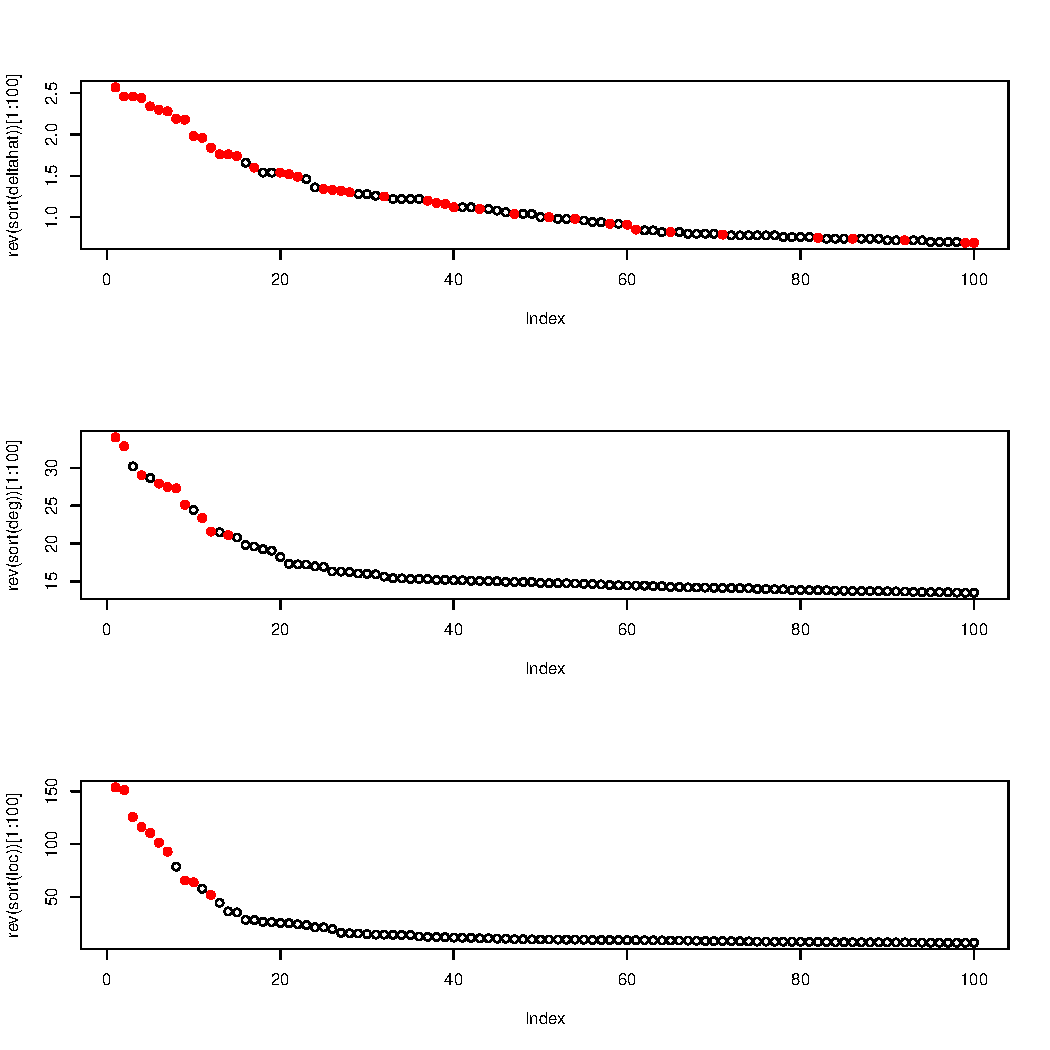
\includegraphics[width=.9\linewidth]{subspacerecovery}
\caption{we can approximate low dimensional subspaces
}
\label{fig:Lhat}
\end{figure}




% section results (end)


\section{Discussion} % (fold)
\label{sec:discussion}

% section discussion (end)
































% Acknowledgements should only appear in the accepted version. 
\section*{Acknowledgments} 
 


% In the unusual situation where you want a paper to appear in the
% references without citing it in the main text, use \nocite
\nocite{langley00}

\bibliography{/Users/joshyv/Research/misc/biblist}
\bibliographystyle{icml2010}

\end{document} 


% This document was modified from the file originally made available by
% Pat Langley and Andrea Danyluk for ICML-2K. This 2010 version was
% created by Thorsten Joachims & Johannes Fuernkranz, 
% slightly modified from the 2009 version by Kiri Wagstaff and 
% Sam Roweis's 2008 version, which is slightly modified from 
% Prasad Tadepalli's 2007 version which is a lightly 
% changed version of the previous year's version by Andrew Moore, 
% which was in turn edited from those of Kristian Kersting and 
% Codrina Lauth. Alex Smola contributed to the algorithmic style files.  


